\chapter[Activation Functions]{Activation Functions}
\label{ch:activation-functions}\index{activation functions|(}
\citet{caterini2018} defined artificial neural networks as ``a model that would imitate the function of the human brain---a set of neurons joined together by a set of connections. Neurons, in this context, are composed of a weighted sum of their inputs followed by a nonlinear function, which is also known as an activation function.''

Activation functions are used in artificial neural networks to determine whether the output of the neuron should be considered further or ignored. If the activation function chooses to continue considering the output of a neuron, we say that the neuron has been activated. The output of the activation function is what is passed on to the subsequent layer in a multilayer neural network. To determine whether a neuron should be activated, the activation function takes the output of a neuron and transforms it into a value commonly bound to a specific range, typically from 0 to 1 or -1 to 1 depending on the which activation function is applied.

\section{Step Function}\label{sec:step-function}\index{step function}

\begin{marginfigure}
  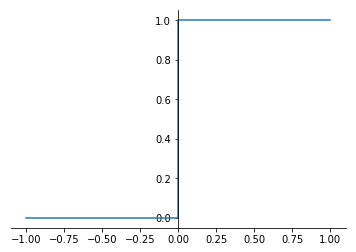
\includegraphics{graphics/activation_functions/step_function.png}
  \caption{
    A graph of the step function. 
  }
  \label{fig:stepfunction}
\end{marginfigure}

\begin{equation}\label{stepfunction}
    f(x) =
    \begin{dcases*}
        0 & \text{for \(x < 0\)} \\
        1 & \text{for \(x \geq 0\)} \\
    \end{dcases*}
\end{equation}

\begin{equation}\label{stepfunctionderivative}
    \frac{d}{d(x)}f(x) =
      \begin{dcases*}
                                       0 & \text{for \(x \neq 0\)} \\
                                       ? & \text{for \(x = 0\)} \\
      \end{dcases*}
\end{equation}

The Heavside step function, visualised in figure~\ref{fig:stepfunction} and defined by equation~\ref{stepfunction}, is one of the simplest activation functions that can be used in a neural network. This function returns 0 if the input of a node is less than a predetermined threshold (typically 0), or otherwise it returns 1 if the output of the node is greater than or equal to the threshold. This activation function was first used in a machine learning context by \citet{rosenblatt1957perceptron} in his seminal work describing the perceptron, the precursor to the modern day neural network. 

Nowadays, the step function is seldom used in practice as it cannot be used to classify more than one class. Furthermore, since the derivative of this function is 0 , as defined by equation~\ref{stepfunctionderivative}, gradient descent algorithms are not be able to progressively update the weights of a network that makes use of this function \citep{Snyman2005}.

\section{Linear Functions}\label{sec:linear-function}\index{linear activation function}

\begin{equation}\label{linearfunction}
    f(x) = ax + b
\end{equation}

\begin{equation}\label{linearfunctionderivative}
    \frac{d}{d(x)}f(x) = a
\end{equation}

A linear activation function, is any function in the format of equation~\ref{linearfunction}, where $a, b \in \mathbb{R}$. This function seeks to solve some of the shortcomings of the step function. The output produced by a linear activation function is proportional to the input. This property means that linear activation functions can be used for multi-class problems. However, linear functions can only be utilised on problems that are linearly separable and can also run into problems with gradient descent algorithms, as the derivative of a linear function is a constant, as seen in equation~\ref{linearfunctionderivative}. Additionally, since the output of the linear function is not bound to any range, it could be susceptible to a common problem when training deep neural networks called the exploding gradient problem, which can make learning unstable \citep{goodfellow2016deeplearning}.

\section{Sigmoid Function}\label{sec:sigmoid}\index{sigmoid function}

\begin{marginfigure}
  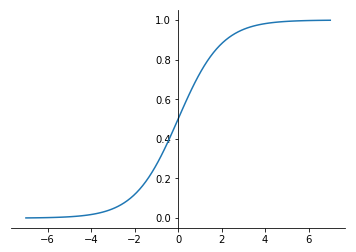
\includegraphics{graphics/activation_functions/sigmoid_function.png}
  \caption{
    A graph of the sigmoid function.
  }
  \label{fig:sigmoidfunction}
\end{marginfigure}

\begin{equation}\label{sigmoidfunction}
    f(x) = \frac{1}{(1 + e^{-x})}
\end{equation}

\begin{equation}\label{sigmoidfunctionderivative}
    \frac{d}{d(x)}f(x) = f(x)(1-f(x))
\end{equation}

The sigmoid function or logistic function, visualised in figure~\ref{fig:sigmoidfunction} and represented by  equation~\ref{sigmoidfunction}, is one of the most commonly used activation functions in neural networks, because of its simplicity and desirable properties. The use of this function in neural networks was first introduced by \citet{DavidE.Rumelhart1986Lrbb}, in one of the most important papers in the field of machine learning, which described the back-propagation algorithm and the introduction of hidden layers, giving rise to modern day neural networks.  The values produced by the sigmoid function are bound between 0 and 1, both not inclusive, which help manage the exploding gradient problem. The derivative of this function, represented by equation~\ref{sigmoidfunctionderivative}, produces a very steep gradient for a relatively small range of values, typically in the range of $-2$ to $2$. This means that for most inputs that the function receives it will return values that are very close to either 0 or 1.

On the other hand, this last property makes the sigmoid function very susceptible to the vanishing gradient problem \citep{bengio94}. When observing the shape of the sigmoid function we see that towards the ends of the curve, the function becomes very unresponsive to changes in the input. In other words, the gradient of the function for large inputs becomes very close to 0. This can become very problematic for neural networks that are very deep in design, such as recurrent neural networks (RNNs).To address this problems in RNNs Long Short-Term Memory (LSTM) units where introduced as a variant of the traditional RNN architecture \citep{hochreiter1997long}.

\section{Hyperbolic Tangent}\label{sec:tanh}\index{hyperbolic tangent}
\begin{marginfigure}
  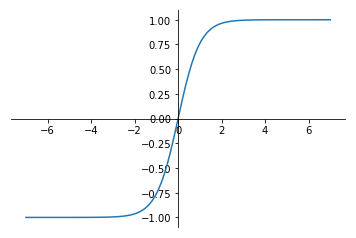
\includegraphics{graphics/activation_functions/tanh_function.png}
  \caption{
    A graph of the hyperbolic tangent (tanh) function.
  }
  \label{fig:tanhfunction}
\end{marginfigure}

\begin{equation}\label{tanhfunction}
    f(x) = \frac{(e^{x} - e^{-x})}{(e^{x} + e^{-x})}
\end{equation}

\begin{equation}\label{tanhfunctionderivative}
    \frac{d}{d(x)}f(x) = 1-f(x)^2.
\end{equation}

The hyperbolic tangent (tanh) function, visualised in figure~\ref{fig:tanhfunction} and represented by equation~\ref{tanhfunction}, is another common activation function that is sometimes used instead of sigmoid. The tanh function has the same characteristics of the sigmoid function mentioned above. In fact, when comparing figure~\ref{fig:sigmoidfunction} to figure~\ref{fig:tanhfunction} one can observe that the tanh function is simply a scaled and translated version of the sigmoid function. As a result of this scaling and translation, the tanh function has a steeper gradient towards the origin, and it returns values between -1 and 1. The derivative of the hyperbolic tangent function is represented by equation~\ref{tanhfunctionderivative}.

\citet{lecun2012efficient} analysed various factors that affect the performance of backpropagation, and suggested that tanh may be better suited than sigmoid as an activation function due to its symmetry about the origin, which is more likely to produce outputs that are on average close to zero, resulting in sparser activations. This means that not all nodes in the network need to be computed, leading to better performance. \citet{glorot2010understanding} studied in detail the effects of the sigmoid and tanh activation functions and noted how the sigmoid function in particular is not well suited for deep networks with random initialisation and go on to propose an alternative normalised initialisation scheme which produced better performance in their experiments.

\section{Rectified Linear Unit}\label{sec:relu}\index{rectified linear unit (relu)}
\begin{marginfigure}
  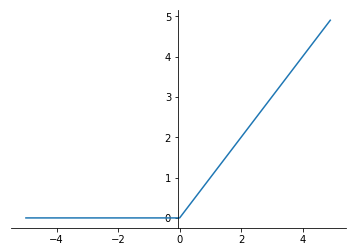
\includegraphics{graphics/activation_functions/relu_function.png}
  \caption{
    A graph of the ReLU function.
  }
  \label{fig:relugraph}
\end{marginfigure}

\begin{equation}\label{relufunction}
    f(x) =
      \begin{dcases*}
                                       0 & \text{for $x < 0$} \\
                                       x & \text{for $x \geq 0$} \\
      \end{dcases*}
\end{equation}

\begin{equation}\label{relufunctionderivative}
    \frac{d}{d(x)}f(x) =
      \begin{dcases*}
                                       0 & \text{for $x < 0$} \\
                                       1 & \text{for $x \geq 0$} \\
      \end{dcases*}
\end{equation}

The Rectified Linear Unit (ReLU) function, visualised in figure~\ref{fig:relugraph} and represented by  equation~\ref{relufunction}, returns 0 if the input of the function is negative, otherwise it outputs the value of the input itself. This function is non-linear in nature even though at first glance it may seem similar to an identity function. The ReLU function is becoming one of the more commonly used activation functions due to its simplicity, performance, and suitability to networks with many layers. Another benefit of the ReLU function is that it produces sparse activations unlike many other commonly used functions such as the sigmoid. 

The ReLU function has been used in many neural network models to improve their performance. \citet{Nair2010} use ReLU to improve the performance of Restricted Boltzmann Machines in object recognition. \citet{KrizhevskyAlex2017Icwd} introduced a breakthrough Convolutional Neural Network (CNN) architecture called AlexNet, which pioneered the use of the ReLU activation function together with dropout layers to minimise over fitting in CNNs. 

Unfortunately, because the gradient of the function for inputs that are negative is 0, as seen in equation~\ref{relufunctionderivative}, the ReLU function can still be susceptible to the vanishing gradient problem. To manage this problem a variant of the ReLU function, called Leaky ReLU is sometimes used. Rather than simply returning 0 for negative inputs, the leaky ReLU returns a very small value such as $0.01x$. \citet{maas2013rectifier} compared the performance of Sigmoid, ReLU and Leaky ReLU functions and found that while the the performance of both the ReLU and Leaky ReLU functions was better than the performance achieved with the sigmoid function, the performance of the two ReLU functions was nearly identical.
\index{activation functions|)}
